
\section{Implementering}
\subsection{Model}
Modellen er nu lavet så det er muligt at vælge mere end én spiller. I både \textit{GameSingleplayer} og \textit{GameMultiplayer} findes en timer hvor det dog kun er i Singleplayer-spillet at timerens opdateringsinterval formindskes efter hvert femte samlet æble. Slangen er stadig defineret som en ArrayList i klassen \textit{Snake}, hvor bl.a. dens retning defineret ved en 'Direction'-enum er og en 'move'-metode. 
\linebreak

I spil-klasserne oprettes en eller to \textit{Snake}-objekter og et \textit{Board}-objekt med en given højde og bredde. Der oprettes også et \textit{Timer}-objekt, der opdaterer slangens bevægelse med et vis tidsinterval imellem hver opdatering.  
\linebreak

Game-klasserne har også en 'move'-metode hver, som kaldes med en 'Direction' som parameter af klassernes tilhørende control-klasser, \textit{BoardSingleplayerListener} eller \textit{BoardMultiplayerListener} - når en a piletasterne (player 1) eller (A, S, W, D) (player 2) trykkes ned. I denne metode tjekkes der, om slangen spiser sig selv igennem dens metode 'isNeckDirection'. Denne metode tjekker om den givne retning 'direction' er lig med 'getOppositeOf' den nuværende retning, 'headDirection'. 'getOppositeOf' er \textit{Direction}-klassens metode, der tager en Direction som parameter, og returnerer den modsatte Direction. Returnerer 'isNeckDirection' true, gås der ud af 'move'-metoden igen, og spillet venter på det næste input. Returnerer den false fortsætter 'move'-metoden med metoden 'isBoardFull', der tjekker om det er det er den sidste frie plads i banen ved at sammenligne banens størrelse og slange-ArrayListens størrelse. I dette tilfælde har spilleren vundet.
\linebreak

Der oprettes også et felt, 'newHeadPosition', der oprettes ved at kalde på 'Snake'-klassens metode 'getNextHeadPosition', som tager 'direction' og 'board' som parametre. Her beregnes den nye række og kolonne for hovedet, hvis den bevæger sig i den givne retning. 'board' kalder på sin 'wrap'-metode, der tager den nye positions række og kolonne som parametre. \textit{Board}-objektet repræsenterer banen ved at have en længde og en højde målt ved rækker og kolonner. Denne har metoden 'wrap', der tjekker om den givne række og kolonne ligger inden for banens størrelse. Hvis ikke, returnerer den et nyt Field med en række eller kolonne, der ligger i den modsatte del af banen. Ligger feltet inde på banen, returnerer den blot et nyt felt med de samme koordinater.
\linebreak

Der undersøges nu med det nye felt om det har samme koordinater som et oprettet 'Food'-objekt, der oprettes på samme måde som i den simple version af spillet. Denne boolean bruges i \textit{Snake}-klassens egen 'move'-metode. I denne metode tjekkes først om den ny-beregnede hovedposition har samme koordinater som en del af kroppen. I dette tilfælde returnerer metoden true, spillet stopper og spilleren har tabt. Ellers fjernes det sidste element i slangens ArrayListe (halen), hvis slangen \textit{ikke} spiser \textit{Food}-objektet, mens den tilføjer et nyt hoved på index 0 uanset om den spiser \textit{Food}-objektet eller ej.
\linebreak 
   
Specielt for multiplayer-spillet tjekkes der også om den en slange 

\subsubsection{Multiplayer}

\subsection{View (Brugergrænseflade)}
Ændret siden simpel: Tilføjede scener. Brug af importerede billeder. Optegning af slange efter bevægelse.

Når \textit{View}-klassen konstrueres, opretter den som tidligere nævnt panel-objekterne fra samme pakke. Derudover opretter den også view-klassen \textit{Audio}, der står for spillets lyde, som spilles efter slangens handlinger i spilscenen hvis klassens Boolean felt 'muted' er falsk. \textit{ViewFrame} kalder først på metoden 'showMenu', der kalder på metoden 'setFrameComponents', som bruges hver gang vinduet skal skifte paneler ud. Metoden fjerner først alle sine komponenter, tager to nye komponenter som parameter, og placerer den førstnævnte øverst i sit BorderLayout, og det andet komponent i midten - dvs. nedenunder. Når 'showMenu' kaldes, sættes \textit{HeaderBasePanel}-objektet som det øverste panel, mens \textit{MenuPanel} er panelet under. \textit{HeaderBasePanel} viser en topbar, som indeholder spillets titel, tastatur-genveje og en JButton, som viser om lyden er slået til eller fra og som også kan bruges til at slå lyden til eller fra. \textit{ViewMenu}-panelet indeholder JButtons som giver spilleren adang til spillets scener: Singleplayer, Multiplayer og Controls - der fører til hjælpescenen \textit{ControlsPanel}. Desuden har den også en \textit{Quit}-knap, som fungerer som vinduets kryds i hjørnet. 

Da \textit{ViewFrame} bruger BorderLayout, er det simpelt at placere et header-panel øverst, og det ønskede scene-panel nedenunder. Alle andre view-klasser er efterladt med standard-layoutet \textit{FlowLayout}, da deres komponenter skal placeres i specifikke koordinater. Dette gøres med \textit{setLocation} der definerer komponentets præcise placering ved x- og y-koordinater. Når spilleren ændrer vinduets størrelse, er deres koordinater dog ikke altid bevaret hvis komponenterne f.eks. altid skal ligge i midten af vinduet, eftersom punktet (0,0) ændres, idet den følger vinduets venstre hjørne. Disse kald på \textit{setLocation}-metoden er derfor placeret i panelernes \textit{paintComponent}-metode da, denne køres hver gang vinduet skaleres. Koordinaterne beregnes derved påny hver gang vinduet skaleres, og komponenterne kan derfor altid få de rigtige koordinater. Denne metode er brugt til alle billeder, JComponents og al tekst der oprettes eller tegnes.

I klassen \textit{OptionsBasePanel} tegnes grafikken til spil-delen. Her er lagt specielt vægt på, at felternes størrelse passer til spillerens ønskede bane-størrelse og spillerens ønskede vinduesstørrelse samtidig med at bevare dens kvadrate form, der jo ikke var tilfældet i den simple version. Metoden `getFieldSideLength' beregner ud fra disse to størrelser den størst mulige længde og højde af et enkelt felt og returnerer derefter den mindste af de to værdier. På denne måde kan feltet være kvadratisk og passer med sikkerhed på begge led af vinduet. Denne 'getFieldSideLength'-metode kan nu bruges til at bestemme størrelsen af og tegne banen, slangen og æblet, så de passer til vinduets størrelse. Da disse tegnemetoder bliver kaldt fra 'paintComponent'-metoden, der køres igennem konstant under spillet og når vinduesstørelsen ændres, kan spilleren udvide vinduet for at se spillet i en større version, der uafhængigt af vinduesskaleringen, skaleres lige meget på begge led.

\subsubsection{Tegning af slangen}
Udover bane-størrelse er det også muligt at vælge slangens farve. Når en farve er valgt tjekkes der i 'drawSnake'-metoden i \textit{OptionsBasePanel}-klassen om farven har været valgt før. Hvis ikke tilføjes den nye farve til ArrayListen 'snakeColors' i metoden 'addSnakeColor'. Denne metode farver også alle billederne, som viser slangens dele og tilføjer den til delens egen ArrayListe. F.eks. er 'snakeHeadUp' en ArrayListe, som indeholder alle de brugte farveversioner af 'snakeHeadUp'-billedet. Farvningen af billederne sker igennem 'colorSnakeImage'-metoden, der tager et BufferedImage og et 'Color'-objekt som parametre. Her oprettes der et WritableRaster-objekt, der gør det muligt at manipulere med et billedets pixel. Dette gøres ved at kopiere billedet med BufferedImages 'copyData'-metode, og parameteren null, hvilket opretter en kopi af billedets areal som en rektangel og ind i et passende WritableRaster-objekt. I for-løkken undersøges om den valgte pixel har farven på øjnene, da den så ikke skal farves. Dette gøres med billedets 'getRGB'-metode i et if-statement og den fundne farvekode for øjenene. Farvekoden er bestemt ved at printe alle farvekoderne for et billede af slangens hoved, og derefter finde den farvekode, som forekommer mest sjældent. I if-statementet farves slangen ved at der oprettes et array af heltal, der skal holde på R-, G- og B-værdierne for den valgte pixel. Denne defineres ved at bruge 'getPixel'-metoden på WritableRaster-objektet, der giver et heltals-array med størrelsen tre, der kan tildeles den nye farves RGB-værdier og derefter bruges til at farve den valgte pixel, med metoden 'setPixel', der tager imod koordinaterne og farvearrayet. Endeligt, returner 'colorSnakeImage'-metoden et nyt BufferedImage, der nu er farvet og kan tilføjes til kropsdelens array.
\linebreak

Har den valgte farve været valgt tidligere, bestemmes dens index i 'snakeColors'-ArrayListen, som kan bruges til at hente alle de rigtige farveversioner af slangens dele. På denne måde behøver billederne ikke at blive farvet en bestemt farve mere end én gang. Efter at have fundet billederne for slangen i den rigtige farve, skaleres alle billederne, så de passer til bane-størrelsen. 
\linebreak

I Simpel Snake kan spilleren ud fra slangens krop se hvor han har været, men ikke hvilken vej han har bevæget sig, idet de udfyldte felter er fyldt helt ud til kanten. Slangens udseende forbedres derfor ved at vise slangens bevægelsesretning og retningsskift i hver enkel del af dens krop og generelt erstatte alle firkanterne, med mere beskrivende billeder. Dette giver seks mulige udseender for hver enkel del af slangens krop. Hovedet og enden af halen, findes hver i fire versioner afhængig af retningen, som spilleren vælger for hovedet, eller retningen af kropsdelen lige før halen. Kropsstykkerne imellem er dog ikke kun afhængig af retningen af stykket lige før eller lige efter, men begge dele. Den vandrette del og den lodrette del af slangen bestemmes let ved at undersøge om stykket, der skal tegnes ligger i samme række eller kolonne som stykkerne før og efter. Slangens hjørnestykker bestemmes på en mere indviklet måde, da stykket og dens tilgrænsende stykker aldrig ligger i samme række eller kolonne, men derimod kan ligge i fire forskellige forhold til hinanden (Se figur 2.2). I figur \ref{fig:corner1} ligger de tilgrænsende felter lige under og til højre for hjørnet, men dette gælder f.eks. ikke for figur \ref{fig:corner3} hvor det ene stykke ligger lige under, mens det andet stykke ligger til venstre for hjørnet uden at grænse op til dens venstre side, der ellers ville give hjørnestykket spejlvendt i y-aksen. Da felterne for kroppen ligger i en Array-liste sorteret efter slangens opnåede dele, sammenlignes et felt med feltet før og efter det i listen. Da stykket foran og bagved uden påvirkning på hjørnestykket kan bytte plads, findes der altså otte situationer for et enkelt hjørnestykke. I alt tjekkes der derfor - for kroppen alene - 34 mulige forhold mellem et stykke og dens to tilgrænsende stykker.
\linebreak

I \textit{BoardBasePanel}-klassen blev der undersøgt alle de mulige situationer hvorpå slangen kan se ud. Passede den valgte kropsdels forhold til delen foran og bagved med et if-statement, blev kropsdelens billede skiftet ud med det passende billede og derefter tegnet for den del. Det har dog været meget langt, da et if-statement for ét billede af et hjørne alene tog flere linjer, men koden kunne simplificeres ved at finde et mønster i de fire if-statements. 
'isSnakeCorner'-metoden returnerer en boolean 'isCorner', som fortæller om tre \textit{Field}-objekter udgør et specifikt hjørne. Et if-statement før indeholdte alle situationer opdelt med ||-symbolet, men er nu erstattet af fire korte if/else statements med 12 forskellige variable, der gør det muligt kun at kalde én boolean. Programmet kører ikke alle if-else-statements igennem hver gang den skal lave et hjørne, men kun det hjørne som bliver kaldt. Variablerne kan enten have værdien 0, 1, -1, 'lastColumn' eller 'lastRow'. Da det specifikke hjørne skal dukke op et bestemt sted alt efter hvor på banen slangen befinder sig.
\linebreak

De første to rækker kode af \textit{isCorner}-metoden, bruges når slangen er placeret midt på banen (se figur \ref{fig:corner1}), og derved grænser op til sin foran- (front) og bagvedliggende del (front og back). Disse dele findes enten ved getColumn()+1 eller getColumn()-1 og på samme måde getRow()+1 eller getRow()-1. De to næste lijner kode i \textit{isCorner} beskriver, slangens placerering på den sidst række (altså i bunden af banen) og går gennem torussen, så noget af den ender øverst i banen (se figur \ref{fig:corner2}).
De to næste linjer kode er på samme måde, slangens placering yderst til højre og går gennem torussen (se figur \ref{fig:corner3}) hvorefter noget af den ender på den modsatte side.
De to sidste linjer kode er til, slangens bevægelse igennem torussen to steder i et af hjørnerne. Altså hvis slangen f.eks. er nede i højre hjørne, går gennem torussen ved at gå ned ad, og straks til højre gennem torussen igen (se figur \ref{fig:corner4}).
Derved er alle hjørne-situationer gennemgået.
Man kan se et mere detaljeret billede af snake-kroppen i Appendix (Bilag A).
\begin{figure}[h]
	\centering
	\graphicspath{ {pics/} }
	\caption{}
	\subfloat[Corner 1]{\label{fig:corner1}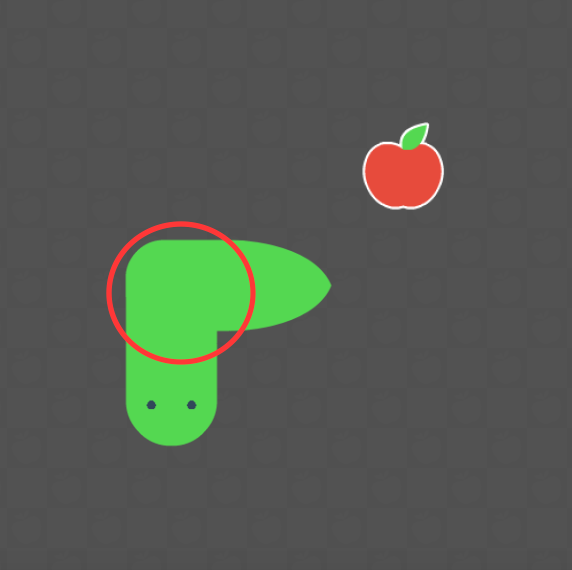
\includegraphics[width=0.15\textwidth]{Corner1.png}}
	\hspace{0.05\textwidth}
	\subfloat[Corner 2]{\label{fig:corner2}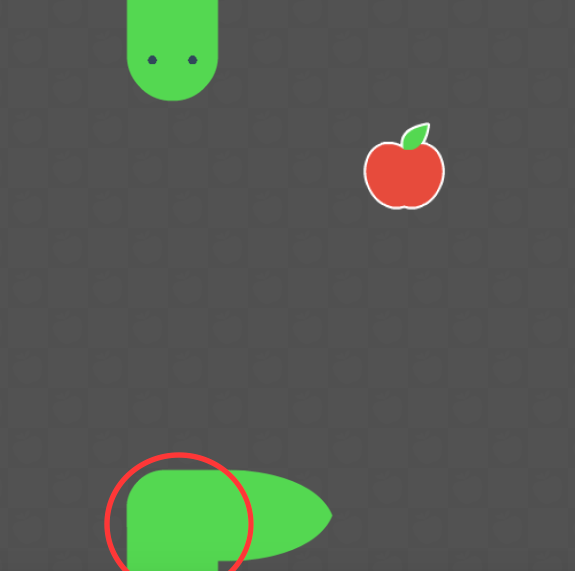
\includegraphics[width=0.15\textwidth]{Corner2.png}}
	\hspace{0.05\textwidth}
	\subfloat[Corner 3]{\label{fig:corner3}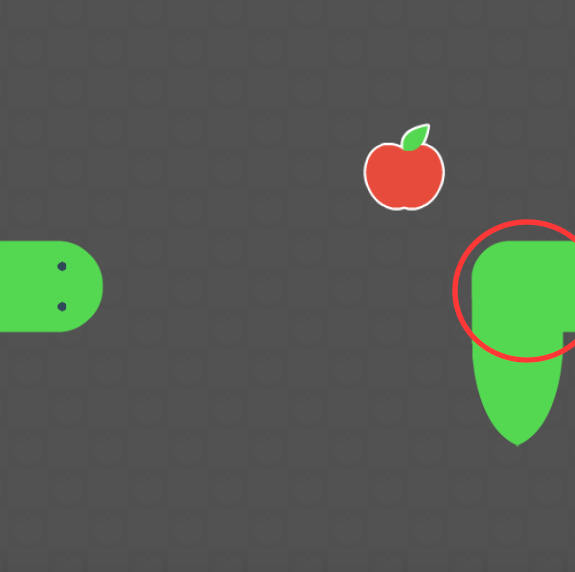
\includegraphics[width=0.15\textwidth]{Corner3.png}}
	\hspace{0.05\textwidth}
	\subfloat[Corner 4]{\label{fig:corner4}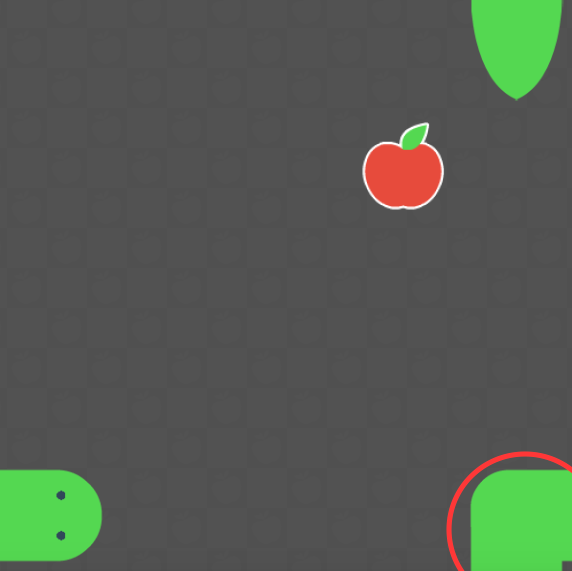
\includegraphics[width=0.15\textwidth]{Corner4.png}}
\end{figure}

Når spilleren færdiggør spillet enten ved at tabe eller vinde, tegnes Game Over-skærmen ved en gennemsigtig rektangel, tekst og JButtons, der giver mulighed for at gå tilbage til menuen eller spille igen.

\subsection{Control (Styring)}
Ændret siden simpel: Mute. Pause. Return. Return to Menu. Start/Play Again.
\linebreak

For at give spilleren valgfrihed er der til mange funktioner både implementeret en JButton og en tilhørende genvej gennem tastaturet. Fra tastaturet er der blevet implementeret genvejene: (M) - mute, (P) - pause, (Esc) return to menu, (Backspace) - return og (Enter/Space) - start / play again. Control-klasserne nedarver fra KeyAdapter-klassen, der registrerer tastatur-input. Samtidig implementerer den ActionListener-klassen, der registrerer tryk på JButtons. Disse klasser tilføjer KeyListeners til \textit{ViewFrame}-klassen, og ActionListeners til hver enkel knap, der har funktioner i ActionListenerens tilhørende control-klasse. Individuel kontrol over de forskellige knapper fås ved at sætte en unik ActionCommand til hver enkel knap, der derefter kan tjekkes for i ActionListeneren abstrakte metode 'actionPerformed'. Det er her også nødvendigt efter knappetryk at bruge 'requestFocus'-metoden på \textit{ViewFrame}-klassen, da spillet efter knappetryk, får et nyt fokus, hvilket betyder, at tastatur-inputtet ikke opfattes af spillet.
Især når \textit{ViewFrame} oprettes, bruges 'setFocusable'- og 'requestFocus'-metoderne, eftersom tastatur-input allerede skal være brugbart når spillet åbnes på grund af 'mute'-funktionen.
\linebreak

\textit{ViewFrameListener}-klassen er som tidligere nævnt en global klasse, der står for kontrollen overalt i spillet. Dvs. muligheden for at slå lyden til eller fra eller vende tilbage til menuen. Når enten (M) eller lydknappen trykkes på, sættes \textit{Audio}-klassens boolean 'mute' til det modsatte af det den i forvejen var, mens \textit{HeaderBasePanel} (eller dens underklasser) notificeres for at opdatere lyd-ikonet. [INSERT PIC]
\linebreak

\textit{BoardSingleplayerListener} og \textit{BoardMultiplayerListener} indeholder metoden 'actionPerformed', der genstarter eller går ud af spillet når spilleren trykker på 'Play Again'-knappen eller 'Menu'-knappen. Klasserne indeholder også KeyEvents, som kalder på en 'move'-metode i \textit{GameSingleplayer} eller \textit{GameMultiplayer}, der får slangen til at bevæge sig, når spilleren trykker på tastatur-tasterne, som styrer slangen. Klasserne indeholder også KeyEvents'ene (P), der fryser eller ''af-fryser'' spillet og (ENTER)/(SPACE), der fungerer som 'Play Again' knappen.
\linebreak

\textit{OptionsListener}, der er en abstrakt klasse implementeret af \textit{OptionsSingleplayerListener} og \textit{OptionsMultiplayerListener}, styrer knapperne i indstillings-scenerne. Før spillets start kan spilleren som tidligere nævnt - udover at vælge farve og sværhedsgrad - vælge banestørrelsen defineret med 'width' og 'height', der beskriver helholdsvis antal felter hen ad x-aksen og antal felter op ad y-aksen. Denne funktion er indbygget vha. to 'JFormattedTextFields', der har fået en 'Formatter', som begrænser inputtet til højst et tre-cifret tal. Dette begrænser spillerens mulighed for at indtaste en ugyldig størrelse. Da tekstfelterenes Formatter får deres caret til at sætte sig i starten af tekstfeltet selvom spilleren trykker et andet sted i feltet, implementerer \textit{OptionsBasePanel}-klassen en FocusListener, der har de abstrakte metoder 'focusGained' og 'focusLost'. I 'focusGained' bruges SwingUtilities 'invokeLater'-metode, der sørger for at opgaver ikke udføres samtidig så brugergrænsefladen kan opdateres korrekt.
\linebreak

Trykkes på en af farve-knapperne eller sværhedsgrads-knapperne, optegnes den vha. JButton-metoden 'setBorder' med en tyk kant, for at vise at den er aktiv, mens kanterne på de andre knapper fjernes med 'setBorderPainted(false)'. Trykkes på en farveknap, sendes farven til \textit{BoardSingleplayerPanels} eller \textit{BoardMultiplayerPanels} 'setSnakeColor'-metode, der derefter bruger farven som beskrevet tidligere. Trykkes på en sværhedsgradsknap, sættes  en 'Difficulty' enum i superklassen til den valgte sværhedsgrad, hvorefter denne bruges når 'Play'-knappen i underklasserne trykkes eller der trykkes (ENTER). 'Play'-knappen kalder på den implementerede abstrakte metode 'playAgain', som først tjekker om tekst-felterne for bane-størrelsen er tomme, da der så printes en fejlmelding. For ikke at gøre det for svært for spilleren at indtaste en gyldig værdi, ses der bort fra eventuelle mellemrum før, i eller efter tallene. Dette gøres med metoden 'getInput' i superklassen, der fjerner alle mellemrum. Der undersøges derefter om tallene ligger mellem 5 og 100. Hvis dette er tilfældet, sættes bane-størrelsen vha. game-klassernes 'setBoardSize'-metode, sværhedsgraden sættes med 'setTimedMovementSpeed'-metoden med et heltals-parameter afhængig af Difficulty enum-staten. Til sidsts startes spillet med metoden 'start' og \textit{ViewFrame}-klassens 'showGame' metode kaldes for at skifte options-panelet ud med spil-panelet.